% Asistencia de IA (Codex): integración de notas, síntesis provisional y maquetación.
% Compilar desde la raíz con pdflatex notas/notas.tex, biber notas y dos pdflatex.
\documentclass[10pt,a4paper]{article}
\usepackage[T1]{fontenc}
\usepackage{lmodern}
\usepackage[american,spanish,es-noshorthands,es-tabla,es-nodecimaldot,es-noquoting]{babel}
\usepackage{csquotes}
\usepackage{graphicx,booktabs,tabularx}
\usepackage[margin=2.3cm]{geometry}
\usepackage[backend=biber,style=ieee,language=american,autolang=other]{biblatex}
\addbibresource{referencias.bib}
\setlength{\parindent}{0pt}
\setlength{\parskip}{0.35em}
\emergencystretch=1em

\begin{document}
\begin{center}
  {\Large\bfseries Notas de exposición}\\[0.3em]
  {\large Spotify como sistema distribuido en la nube}\\[0.3em]
  Aplicaciones Distribuidas (ISR-701) · UTEQ · Séptimo nivel, paralelo B
\end{center}

% =====================================================================
% Notas: Apartado 1 (Presentación del sistema) y Apartado 2 (Arquitectura)
% Responsable y expositor: Apunte Pazmiño Washington German
% Se incluye en notas/notas.tex con
% % =====================================================================
% Notas: Apartado 1 (Presentación del sistema) y Apartado 2 (Arquitectura)
% Responsable y expositor: Apunte Pazmiño Washington German
% Se incluye en notas/notas.tex con
% % =====================================================================
% Notas: Apartado 1 (Presentación del sistema) y Apartado 2 (Arquitectura)
% Responsable y expositor: Apunte Pazmiño Washington German
% Se incluye en notas/notas.tex con
% \input{notas/apartados/presentacion_arquitectura}
% Claves del .bib: spotifyAbout2026, spotifyQ32026, vansteen2023ds,
%   strid2023fleet, khlebnikova2024dataplatform, spotifyIncident2025,
%   gustavsson2023fleet, soylemez2022microservices
% Asistencia de IA (Claude): borrador revisado contra las fuentes y
%   reescrito con mis palabras.
% =====================================================================

\subsection*{Apartado 1: Presentación del sistema (expone Washington Apunte, 1 min)}

Spotify sirve para descubrir, organizar y escuchar música, pódcasts y
audiolibros desde una sola app. Tiene más de 100 millones de canciones y
8 millones de títulos de pódcast, y está en 184 mercados
\cite{spotifyAbout2026}. Lo usan dos grupos: quienes escuchan gratis con
anuncios y quienes pagan Premium. En el tercer trimestre de 2026 llegó a
788 millones de usuarios activos al mes, 11\,\% más que un año antes. De
ellos, 306 millones son suscriptores Premium y 499 millones usan la
versión con anuncios \cite[p.~3]{spotifyQ32026}.

Con esa escala no basta un servidor, ni siquiera un centro de datos
pequeño. Por eso Spotify es un sistema distribuido y corre en la nube.
La nube, dicho simple, es usar la infraestructura, la plataforma o las
aplicaciones de un proveedor como un servicio: IaaS, PaaS o SaaS
\cite[p.~99]{vansteen2023ds}. Spotify trabaja con Google Cloud desde
2016 y llevó allí su plataforma con \emph{lift and shift}, es decir,
moviendo lo que ya tenía \cite{strid2023fleet}. Antes corría sus
pipelines de datos en un clúster Hadoop propio, el más grande de Europa
\cite{khlebnikova2024dataplatform}.

\subsection*{Apartado 2: Arquitectura (expone Washington Apunte, 2 min)}

\paragraph{Componentes.}
Recorro el diagrama de izquierda a derecha. El usuario pulsa
«reproducir» y la app manda la petición por internet; si no recibe
respuesta, la vuelve a intentar \cite{spotifyIncident2025}. La petición
entra a una región de nube. La primera pieza que la recibe es el
perímetro, hecho con Envoy Proxy, y desde ahí pasa a los servicios de
backend \cite{spotifyIncident2025}. Esos servicios son miles de
componentes en producción, organizados como microservicios
\cite{gustavsson2023fleet}, y cada squad se encarga de los suyos
\cite{strid2023fleet}. Aparte, la app genera eventos de uso. La
plataforma de datos los recoge en colas Pub/Sub y los procesa en
BigQuery, Flink o Dataflow. Son más de un billón de eventos al día y más
de 38\,000 pipelines programados \cite{khlebnikova2024dataplatform}.

\paragraph{La nube en la arquitectura.}
En el diagrama se ven cuatro ideas de nube. La primera son las regiones:
el informe de la caída de 2025 habla de Europa, EE.\,UU. y Asia-Pacífico.
La segunda son los contenedores: Kubernetes ejecuta las instancias del
perímetro, cada una con un límite de memoria. El 16 de abril de 2025
Envoy podía usar más memoria que ese límite; Kubernetes apagaba las
instancias y el ciclo se repetía. Asia-Pacífico siguió funcionando porque
a esa hora tenía menos tráfico \cite{spotifyIncident2025}. La tercera es
la diferencia entre IaaS y PaaS. El \emph{lift and shift} se parece a
IaaS, porque es llevar tu sistema a la infraestructura del proveedor
\cite{strid2023fleet}. La plataforma de datos, en cambio, se apoya en
servicios administrados como Pub/Sub y BigQuery, y eso ya es PaaS
\cite{khlebnikova2024dataplatform}. La cuarta es la gestión a escala: con
Fleet Management, el parche de Log4j llegó al 80\,\% de los servicios de
backend en 9 horas \cite{gustavsson2023fleet}.

\paragraph{Ejemplo propio: SREI.}
SREI es nuestro PFC: un sistema web para registrar los eventos
interculturales de la UTEQ. Tiene un frontend en Angular que llama a una
sola API REST en Spring Boot, con PostgreSQL y los archivos guardados en
la carpeta \texttt{/uploads} del mismo servidor. Es cliente-servidor en
capas, centralizado, y lo desplegamos en local para las pruebas. Nuestro
propio requisito QR-003 pide que funcione sin grandes fallos en los días
laborables, pero si ese servidor se apaga en pleno evento, se cae todo:
es un punto único de fallo. No por eso tocaría copiar los microservicios
de Spotify. Adoptarlos no es trivial y sus retos se deben evaluar según
los requisitos de cada proyecto \cite[p.~1]{soylemez2022microservices}.
Para el tamaño de SREI, yo empezaría por sacar los archivos a un
almacenamiento aparte y usar una base de datos administrada.

% Claves del .bib: spotifyAbout2026, spotifyQ32026, vansteen2023ds,
%   strid2023fleet, khlebnikova2024dataplatform, spotifyIncident2025,
%   gustavsson2023fleet, soylemez2022microservices
% Asistencia de IA (Claude): borrador revisado contra las fuentes y
%   reescrito con mis palabras.
% =====================================================================

\subsection*{Apartado 1: Presentación del sistema (expone Washington Apunte, 1 min)}

Spotify sirve para descubrir, organizar y escuchar música, pódcasts y
audiolibros desde una sola app. Tiene más de 100 millones de canciones y
8 millones de títulos de pódcast, y está en 184 mercados
\cite{spotifyAbout2026}. Lo usan dos grupos: quienes escuchan gratis con
anuncios y quienes pagan Premium. En el tercer trimestre de 2026 llegó a
788 millones de usuarios activos al mes, 11\,\% más que un año antes. De
ellos, 306 millones son suscriptores Premium y 499 millones usan la
versión con anuncios \cite[p.~3]{spotifyQ32026}.

Con esa escala no basta un servidor, ni siquiera un centro de datos
pequeño. Por eso Spotify es un sistema distribuido y corre en la nube.
La nube, dicho simple, es usar la infraestructura, la plataforma o las
aplicaciones de un proveedor como un servicio: IaaS, PaaS o SaaS
\cite[p.~99]{vansteen2023ds}. Spotify trabaja con Google Cloud desde
2016 y llevó allí su plataforma con \emph{lift and shift}, es decir,
moviendo lo que ya tenía \cite{strid2023fleet}. Antes corría sus
pipelines de datos en un clúster Hadoop propio, el más grande de Europa
\cite{khlebnikova2024dataplatform}.

\subsection*{Apartado 2: Arquitectura (expone Washington Apunte, 2 min)}

\paragraph{Componentes.}
Recorro el diagrama de izquierda a derecha. El usuario pulsa
«reproducir» y la app manda la petición por internet; si no recibe
respuesta, la vuelve a intentar \cite{spotifyIncident2025}. La petición
entra a una región de nube. La primera pieza que la recibe es el
perímetro, hecho con Envoy Proxy, y desde ahí pasa a los servicios de
backend \cite{spotifyIncident2025}. Esos servicios son miles de
componentes en producción, organizados como microservicios
\cite{gustavsson2023fleet}, y cada squad se encarga de los suyos
\cite{strid2023fleet}. Aparte, la app genera eventos de uso. La
plataforma de datos los recoge en colas Pub/Sub y los procesa en
BigQuery, Flink o Dataflow. Son más de un billón de eventos al día y más
de 38\,000 pipelines programados \cite{khlebnikova2024dataplatform}.

\paragraph{La nube en la arquitectura.}
En el diagrama se ven cuatro ideas de nube. La primera son las regiones:
el informe de la caída de 2025 habla de Europa, EE.\,UU. y Asia-Pacífico.
La segunda son los contenedores: Kubernetes ejecuta las instancias del
perímetro, cada una con un límite de memoria. El 16 de abril de 2025
Envoy podía usar más memoria que ese límite; Kubernetes apagaba las
instancias y el ciclo se repetía. Asia-Pacífico siguió funcionando porque
a esa hora tenía menos tráfico \cite{spotifyIncident2025}. La tercera es
la diferencia entre IaaS y PaaS. El \emph{lift and shift} se parece a
IaaS, porque es llevar tu sistema a la infraestructura del proveedor
\cite{strid2023fleet}. La plataforma de datos, en cambio, se apoya en
servicios administrados como Pub/Sub y BigQuery, y eso ya es PaaS
\cite{khlebnikova2024dataplatform}. La cuarta es la gestión a escala: con
Fleet Management, el parche de Log4j llegó al 80\,\% de los servicios de
backend en 9 horas \cite{gustavsson2023fleet}.

\paragraph{Ejemplo propio: SREI.}
SREI es nuestro PFC: un sistema web para registrar los eventos
interculturales de la UTEQ. Tiene un frontend en Angular que llama a una
sola API REST en Spring Boot, con PostgreSQL y los archivos guardados en
la carpeta \texttt{/uploads} del mismo servidor. Es cliente-servidor en
capas, centralizado, y lo desplegamos en local para las pruebas. Nuestro
propio requisito QR-003 pide que funcione sin grandes fallos en los días
laborables, pero si ese servidor se apaga en pleno evento, se cae todo:
es un punto único de fallo. No por eso tocaría copiar los microservicios
de Spotify. Adoptarlos no es trivial y sus retos se deben evaluar según
los requisitos de cada proyecto \cite[p.~1]{soylemez2022microservices}.
Para el tamaño de SREI, yo empezaría por sacar los archivos a un
almacenamiento aparte y usar una base de datos administrada.

% Claves del .bib: spotifyAbout2026, spotifyQ32026, vansteen2023ds,
%   strid2023fleet, khlebnikova2024dataplatform, spotifyIncident2025,
%   gustavsson2023fleet, soylemez2022microservices
% Asistencia de IA (Claude): borrador revisado contra las fuentes y
%   reescrito con mis palabras.
% =====================================================================

\subsection*{Apartado 1: Presentación del sistema (expone Washington Apunte, 1 min)}

Spotify sirve para descubrir, organizar y escuchar música, pódcasts y
audiolibros desde una sola app. Tiene más de 100 millones de canciones y
8 millones de títulos de pódcast, y está en 184 mercados
\cite{spotifyAbout2026}. Lo usan dos grupos: quienes escuchan gratis con
anuncios y quienes pagan Premium. En el tercer trimestre de 2026 llegó a
788 millones de usuarios activos al mes, 11\,\% más que un año antes. De
ellos, 306 millones son suscriptores Premium y 499 millones usan la
versión con anuncios \cite[p.~3]{spotifyQ32026}.

Con esa escala no basta un servidor, ni siquiera un centro de datos
pequeño. Por eso Spotify es un sistema distribuido y corre en la nube.
La nube, dicho simple, es usar la infraestructura, la plataforma o las
aplicaciones de un proveedor como un servicio: IaaS, PaaS o SaaS
\cite[p.~99]{vansteen2023ds}. Spotify trabaja con Google Cloud desde
2016 y llevó allí su plataforma con \emph{lift and shift}, es decir,
moviendo lo que ya tenía \cite{strid2023fleet}. Antes corría sus
pipelines de datos en un clúster Hadoop propio, el más grande de Europa
\cite{khlebnikova2024dataplatform}.

\subsection*{Apartado 2: Arquitectura (expone Washington Apunte, 2 min)}

\paragraph{Componentes.}
Recorro el diagrama de izquierda a derecha. El usuario pulsa
«reproducir» y la app manda la petición por internet; si no recibe
respuesta, la vuelve a intentar \cite{spotifyIncident2025}. La petición
entra a una región de nube. La primera pieza que la recibe es el
perímetro, hecho con Envoy Proxy, y desde ahí pasa a los servicios de
backend \cite{spotifyIncident2025}. Esos servicios son miles de
componentes en producción, organizados como microservicios
\cite{gustavsson2023fleet}, y cada squad se encarga de los suyos
\cite{strid2023fleet}. Aparte, la app genera eventos de uso. La
plataforma de datos los recoge en colas Pub/Sub y los procesa en
BigQuery, Flink o Dataflow. Son más de un billón de eventos al día y más
de 38\,000 pipelines programados \cite{khlebnikova2024dataplatform}.

\paragraph{La nube en la arquitectura.}
En el diagrama se ven cuatro ideas de nube. La primera son las regiones:
el informe de la caída de 2025 habla de Europa, EE.\,UU. y Asia-Pacífico.
La segunda son los contenedores: Kubernetes ejecuta las instancias del
perímetro, cada una con un límite de memoria. El 16 de abril de 2025
Envoy podía usar más memoria que ese límite; Kubernetes apagaba las
instancias y el ciclo se repetía. Asia-Pacífico siguió funcionando porque
a esa hora tenía menos tráfico \cite{spotifyIncident2025}. La tercera es
la diferencia entre IaaS y PaaS. El \emph{lift and shift} se parece a
IaaS, porque es llevar tu sistema a la infraestructura del proveedor
\cite{strid2023fleet}. La plataforma de datos, en cambio, se apoya en
servicios administrados como Pub/Sub y BigQuery, y eso ya es PaaS
\cite{khlebnikova2024dataplatform}. La cuarta es la gestión a escala: con
Fleet Management, el parche de Log4j llegó al 80\,\% de los servicios de
backend en 9 horas \cite{gustavsson2023fleet}.

\paragraph{Ejemplo propio: SREI.}
SREI es nuestro PFC: un sistema web para registrar los eventos
interculturales de la UTEQ. Tiene un frontend en Angular que llama a una
sola API REST en Spring Boot, con PostgreSQL y los archivos guardados en
la carpeta \texttt{/uploads} del mismo servidor. Es cliente-servidor en
capas, centralizado, y lo desplegamos en local para las pruebas. Nuestro
propio requisito QR-003 pide que funcione sin grandes fallos en los días
laborables, pero si ese servidor se apaga en pleno evento, se cae todo:
es un punto único de fallo. No por eso tocaría copiar los microservicios
de Spotify. Adoptarlos no es trivial y sus retos se deben evaluar según
los requisitos de cada proyecto \cite[p.~1]{soylemez2022microservices}.
Para el tamaño de SREI, yo empezaría por sacar los archivos a un
almacenamiento aparte y usar una base de datos administrada.


\subsection*{Apartados 3 y 5. Transparencias y comunicación (Jilmar Cedeño, 3 min)}
\textit{Síntesis de las diapositivas para revisión del expositor.}
La app permite elegir la calidad del audio sin seleccionar una región. El
perímetro se encarga de dirigir el tráfico. La caché local permite reproducir
algunas pistas sin conexión \cite{spotifyLossless2025,spotifyIncident2025,spotifyOffline2024}.
En la búsqueda pública, una solicitud HTTPS recibe los resultados en JSON.
Los eventos de uso siguen otro flujo. Pub/Sub separa su publicación de su
procesamiento posterior \cite{spotifyWebApiSearch,khlebnikova2024dataplatform}.

\subsection*{Apartados 4 y 7. CAP, PACELC y comparación (Elian Mendoza, 3 min)}
\textit{Se incluye su borrador técnico. El análisis específico de Spotify y
la comparación con otro sistema están pendientes en ese aporte.}
\begingroup
\let\subsection\subsubsection
% =====================================================================
% Notas técnicas: Apartado 4 (CAP y PACELC) y Apartado 7 (Postura crítica)
% Responsable y expositor: Mendoza Villarroel Elian Jossue
% Se incluye en notas/notas.tex con % =====================================================================
% Notas técnicas: Apartado 4 (CAP y PACELC) y Apartado 7 (Postura crítica)
% Responsable y expositor: Mendoza Villarroel Elian Jossue
% Se incluye en notas/notas.tex con % =====================================================================
% Notas técnicas: Apartado 4 (CAP y PACELC) y Apartado 7 (Postura crítica)
% Responsable y expositor: Mendoza Villarroel Elian Jossue
% Se incluye en notas/notas.tex con \input{notas/apartados/cap_comparacion}
% Claves del .bib: ahmed2023consistency, lee2023consistency,
%                  gilbert2012perspectives, lima2023causal
% Versión inicial: falta el sistema analizado, la comparación y el aporte al PFC.
% =====================================================================

\subsection*{Notas técnicas: CAP y PACELC}

\paragraph{Teorema CAP.}
El teorema CAP establece un compromiso fundamental entre tres propiedades de
los sistemas distribuidos replicados: consistencia, disponibilidad y
tolerancia a particiones \cite[p.~172]{ahmed2023consistency}. Cuando ocurre
una interrupción en la comunicación entre sus nodos, no es posible garantizar
simultáneamente la consistencia y la disponibilidad. Por esta razón, si el
sistema debe seguir funcionando a pesar de una partición de red, tendrá que
priorizar una de estas dos propiedades \cite[p.~2]{lee2023consistency}.

\paragraph{Consistencia (C).}
En el sentido de CAP, la consistencia fuerte exige que las operaciones se
observen como si ocurrieran en una sola copia y en un orden compatible con
el tiempo real \cite[Sec.~2]{gilbert2012perspectives}. Se trata de una
propiedad de seguridad: las respuestas deben respetar esa garantía
\cite[Sec.~1]{gilbert2012perspectives}.

\paragraph{Disponibilidad (A) y tolerancia a particiones (P).}
La disponibilidad es la capacidad de responder a las solicitudes de los
usuarios que leen o modifican el estado compartido
\cite[p.~2]{lee2023consistency}. La tolerancia a particiones parte de que la
comunicación entre servidores no es fiable: los mensajes pueden retrasarse o
perderse y los servidores pueden quedar divididos en grupos que no se
comunican \cite[Sec.~2]{gilbert2012perspectives}.

\paragraph{Comportamiento durante una partición.}
Cuando una réplica rechaza una solicitud o no responde dentro del tiempo de
espera, la base de datos debe decidir entre devolver un resultado
posiblemente obsoleto, sacrificando la consistencia, o informar que el
servicio no está disponible. Los sistemas CP, como HBase o BigTable,
renuncian a la disponibilidad; los sistemas AP, como Cassandra, Dynamo o
Riak, relajan la consistencia \cite[p.~172]{ahmed2023consistency}.

\paragraph{Teorema PACELC.}
PACELC plantea dos decisiones en sistemas replicados. Si hay una partición,
el compromiso es entre disponibilidad y consistencia. Si no hay una
partición, el compromiso es entre latencia y consistencia
\cite{ahmed2023consistency}. Un caso del segundo compromiso es el acceso
causal en almacenamiento georreplicado, donde esperar a que se sincronicen
las réplicas puede retrasar el acceso \cite{lima2023causal}.

\subsection*{Postura crítica}

Priorizar consistencia o disponibilidad depende de lo que necesite cada
aplicación. En un cruce controlado por vehículos autónomos conviene la
consistencia, porque todos deben compartir la misma información antes de
avanzar; en cambio, en el sistema de frenado conviene la disponibilidad,
porque la reacción tiene que ser inmediata
\cite[pp.~2--3]{lee2023consistency}. En una tienda en línea, una consulta
puede devolver datos desactualizados, mientras que la compra requiere
consistencia para que el pedido refleje lo que eligió el cliente
\cite[Sec.~4.4]{gilbert2012perspectives}. En consecuencia, ningún sistema es
superior en todos los casos: cada uno equilibra estas propiedades según su
propósito.

% Pendiente para próximos commits:
%  - Sistema analizado: qué prioriza con y sin partición, clasificación
%    PACELC y ejemplo técnico de su documentación oficial.
%  - Comparación con un segundo sistema real (tabla del apartado 7).
%  - Aporte al PFC para el apartado 8.

% Claves del .bib: ahmed2023consistency, lee2023consistency,
%                  gilbert2012perspectives, lima2023causal
% Versión inicial: falta el sistema analizado, la comparación y el aporte al PFC.
% =====================================================================

\subsection*{Notas técnicas: CAP y PACELC}

\paragraph{Teorema CAP.}
El teorema CAP establece un compromiso fundamental entre tres propiedades de
los sistemas distribuidos replicados: consistencia, disponibilidad y
tolerancia a particiones \cite[p.~172]{ahmed2023consistency}. Cuando ocurre
una interrupción en la comunicación entre sus nodos, no es posible garantizar
simultáneamente la consistencia y la disponibilidad. Por esta razón, si el
sistema debe seguir funcionando a pesar de una partición de red, tendrá que
priorizar una de estas dos propiedades \cite[p.~2]{lee2023consistency}.

\paragraph{Consistencia (C).}
En el sentido de CAP, la consistencia fuerte exige que las operaciones se
observen como si ocurrieran en una sola copia y en un orden compatible con
el tiempo real \cite[Sec.~2]{gilbert2012perspectives}. Se trata de una
propiedad de seguridad: las respuestas deben respetar esa garantía
\cite[Sec.~1]{gilbert2012perspectives}.

\paragraph{Disponibilidad (A) y tolerancia a particiones (P).}
La disponibilidad es la capacidad de responder a las solicitudes de los
usuarios que leen o modifican el estado compartido
\cite[p.~2]{lee2023consistency}. La tolerancia a particiones parte de que la
comunicación entre servidores no es fiable: los mensajes pueden retrasarse o
perderse y los servidores pueden quedar divididos en grupos que no se
comunican \cite[Sec.~2]{gilbert2012perspectives}.

\paragraph{Comportamiento durante una partición.}
Cuando una réplica rechaza una solicitud o no responde dentro del tiempo de
espera, la base de datos debe decidir entre devolver un resultado
posiblemente obsoleto, sacrificando la consistencia, o informar que el
servicio no está disponible. Los sistemas CP, como HBase o BigTable,
renuncian a la disponibilidad; los sistemas AP, como Cassandra, Dynamo o
Riak, relajan la consistencia \cite[p.~172]{ahmed2023consistency}.

\paragraph{Teorema PACELC.}
PACELC plantea dos decisiones en sistemas replicados. Si hay una partición,
el compromiso es entre disponibilidad y consistencia. Si no hay una
partición, el compromiso es entre latencia y consistencia
\cite{ahmed2023consistency}. Un caso del segundo compromiso es el acceso
causal en almacenamiento georreplicado, donde esperar a que se sincronicen
las réplicas puede retrasar el acceso \cite{lima2023causal}.

\subsection*{Postura crítica}

Priorizar consistencia o disponibilidad depende de lo que necesite cada
aplicación. En un cruce controlado por vehículos autónomos conviene la
consistencia, porque todos deben compartir la misma información antes de
avanzar; en cambio, en el sistema de frenado conviene la disponibilidad,
porque la reacción tiene que ser inmediata
\cite[pp.~2--3]{lee2023consistency}. En una tienda en línea, una consulta
puede devolver datos desactualizados, mientras que la compra requiere
consistencia para que el pedido refleje lo que eligió el cliente
\cite[Sec.~4.4]{gilbert2012perspectives}. En consecuencia, ningún sistema es
superior en todos los casos: cada uno equilibra estas propiedades según su
propósito.

% Pendiente para próximos commits:
%  - Sistema analizado: qué prioriza con y sin partición, clasificación
%    PACELC y ejemplo técnico de su documentación oficial.
%  - Comparación con un segundo sistema real (tabla del apartado 7).
%  - Aporte al PFC para el apartado 8.

% Claves del .bib: ahmed2023consistency, lee2023consistency,
%                  gilbert2012perspectives, lima2023causal
% Versión inicial: falta el sistema analizado, la comparación y el aporte al PFC.
% =====================================================================

\subsection*{Notas técnicas: CAP y PACELC}

\paragraph{Teorema CAP.}
El teorema CAP establece un compromiso fundamental entre tres propiedades de
los sistemas distribuidos replicados: consistencia, disponibilidad y
tolerancia a particiones \cite[p.~172]{ahmed2023consistency}. Cuando ocurre
una interrupción en la comunicación entre sus nodos, no es posible garantizar
simultáneamente la consistencia y la disponibilidad. Por esta razón, si el
sistema debe seguir funcionando a pesar de una partición de red, tendrá que
priorizar una de estas dos propiedades \cite[p.~2]{lee2023consistency}.

\paragraph{Consistencia (C).}
En el sentido de CAP, la consistencia fuerte exige que las operaciones se
observen como si ocurrieran en una sola copia y en un orden compatible con
el tiempo real \cite[Sec.~2]{gilbert2012perspectives}. Se trata de una
propiedad de seguridad: las respuestas deben respetar esa garantía
\cite[Sec.~1]{gilbert2012perspectives}.

\paragraph{Disponibilidad (A) y tolerancia a particiones (P).}
La disponibilidad es la capacidad de responder a las solicitudes de los
usuarios que leen o modifican el estado compartido
\cite[p.~2]{lee2023consistency}. La tolerancia a particiones parte de que la
comunicación entre servidores no es fiable: los mensajes pueden retrasarse o
perderse y los servidores pueden quedar divididos en grupos que no se
comunican \cite[Sec.~2]{gilbert2012perspectives}.

\paragraph{Comportamiento durante una partición.}
Cuando una réplica rechaza una solicitud o no responde dentro del tiempo de
espera, la base de datos debe decidir entre devolver un resultado
posiblemente obsoleto, sacrificando la consistencia, o informar que el
servicio no está disponible. Los sistemas CP, como HBase o BigTable,
renuncian a la disponibilidad; los sistemas AP, como Cassandra, Dynamo o
Riak, relajan la consistencia \cite[p.~172]{ahmed2023consistency}.

\paragraph{Teorema PACELC.}
PACELC plantea dos decisiones en sistemas replicados. Si hay una partición,
el compromiso es entre disponibilidad y consistencia. Si no hay una
partición, el compromiso es entre latencia y consistencia
\cite{ahmed2023consistency}. Un caso del segundo compromiso es el acceso
causal en almacenamiento georreplicado, donde esperar a que se sincronicen
las réplicas puede retrasar el acceso \cite{lima2023causal}.

\subsection*{Postura crítica}

Priorizar consistencia o disponibilidad depende de lo que necesite cada
aplicación. En un cruce controlado por vehículos autónomos conviene la
consistencia, porque todos deben compartir la misma información antes de
avanzar; en cambio, en el sistema de frenado conviene la disponibilidad,
porque la reacción tiene que ser inmediata
\cite[pp.~2--3]{lee2023consistency}. En una tienda en línea, una consulta
puede devolver datos desactualizados, mientras que la compra requiere
consistencia para que el pedido refleje lo que eligió el cliente
\cite[Sec.~4.4]{gilbert2012perspectives}. En consecuencia, ningún sistema es
superior en todos los casos: cada uno equilibra estas propiedades según su
propósito.

% Pendiente para próximos commits:
%  - Sistema analizado: qué prioriza con y sin partición, clasificación
%    PACELC y ejemplo técnico de su documentación oficial.
%  - Comparación con un segundo sistema real (tabla del apartado 7).
%  - Aporte al PFC para el apartado 8.

\endgroup

% Asistencia de IA (Codex): síntesis del informe y redacción del borrador.
\subsection*{Apartado 6. Tolerancia a fallos (Melanie Muñoz, 2 min)}

El 16 de abril de 2025, Spotify cambió el orden de sus filtros de Envoy en
todas las regiones. El cambio activó un defecto que derribó las instancias
del perímetro. A las 12:20 UTC saltaron las alarmas por una caída del
tráfico. Los reinicios simultáneos y los reintentos de los clientes
dispararon la carga. Como el máximo de memoria de Envoy superaba el límite
de Kubernetes, las nuevas instancias volvían a detenerse. Asia-Pacífico
soportó el fallo con menos carga. Spotify añadió capacidad para romper el
ciclo, corrigió el defecto y el desajuste de memoria, y anunció mejoras en
los despliegues y el monitoreo \cite{spotifyIncident2025}.

\subsection*{Apartado 8. PFC y conclusiones (Melanie Muñoz, 1 min)}

Washington propone separar los archivos de SREI y migrar PostgreSQL a un
servicio administrado. Así, los archivos y la base de datos dejan de depender
del servidor donde corre la aplicación. Los aportes de Jilmar, Elian y
Melanie quedan pendientes de confirmar.

La distribución regional oculta al usuario la ubicación del servicio, pero
un cambio simultáneo puede propagar el mismo fallo a varias regiones.
Spotify separa la búsqueda por solicitud y respuesta del procesamiento
asíncrono de eventos \cite{spotifyIncident2025,spotifyWebApiSearch,khlebnikova2024dataplatform}.
Para analizar CAP o PACELC hay que identificar qué operación y qué estado
compartido se estudian. La caída de Envoy por sí sola describe un fallo del
perímetro, sin establecer cómo se comporta una réplica ante una partición.


\subsection*{Aportes del equipo}
\begin{tabularx}{\linewidth}{@{}lX@{}}
  \toprule
  \textbf{Integrante} & \textbf{Aportes registrados} \\
  \midrule
  Washington Apunte & Presentación, arquitectura, diagrama, bosquejo, notas y README. \\
  Jilmar Cedeño & Transparencias, comunicación y diagrama de flujo. \\
  Elian Mendoza & Borrador de CAP y PACELC y aportes a la bibliografía. \\
  Melanie Muñoz & Tolerancia a fallos, diagrama causal, sección 8, notas, bitácora y PDF para el SGA. \\
  \bottomrule
\end{tabularx}

\subsection*{Declaración de uso de inteligencia artificial}
Se utilizó Codex para sintetizar el informe oficial de Spotify, preparar el
diagrama de causas raíz, redactar e integrar borradores de las secciones de
Melanie y de las notas, organizar la bitácora a partir de Git y maquetar el
PDF de entrega. Cada integrante debe completar esta declaración con el uso
de IA que corresponda a sus propios aportes.

\renewcommand*{\bibfont}{\footnotesize}
\setlength{\bibitemsep}{0pt}
\printbibliography[title={Referencias citadas}]

\clearpage
\section*{Anexo. Bosquejo de arquitectura}
\begin{center}
  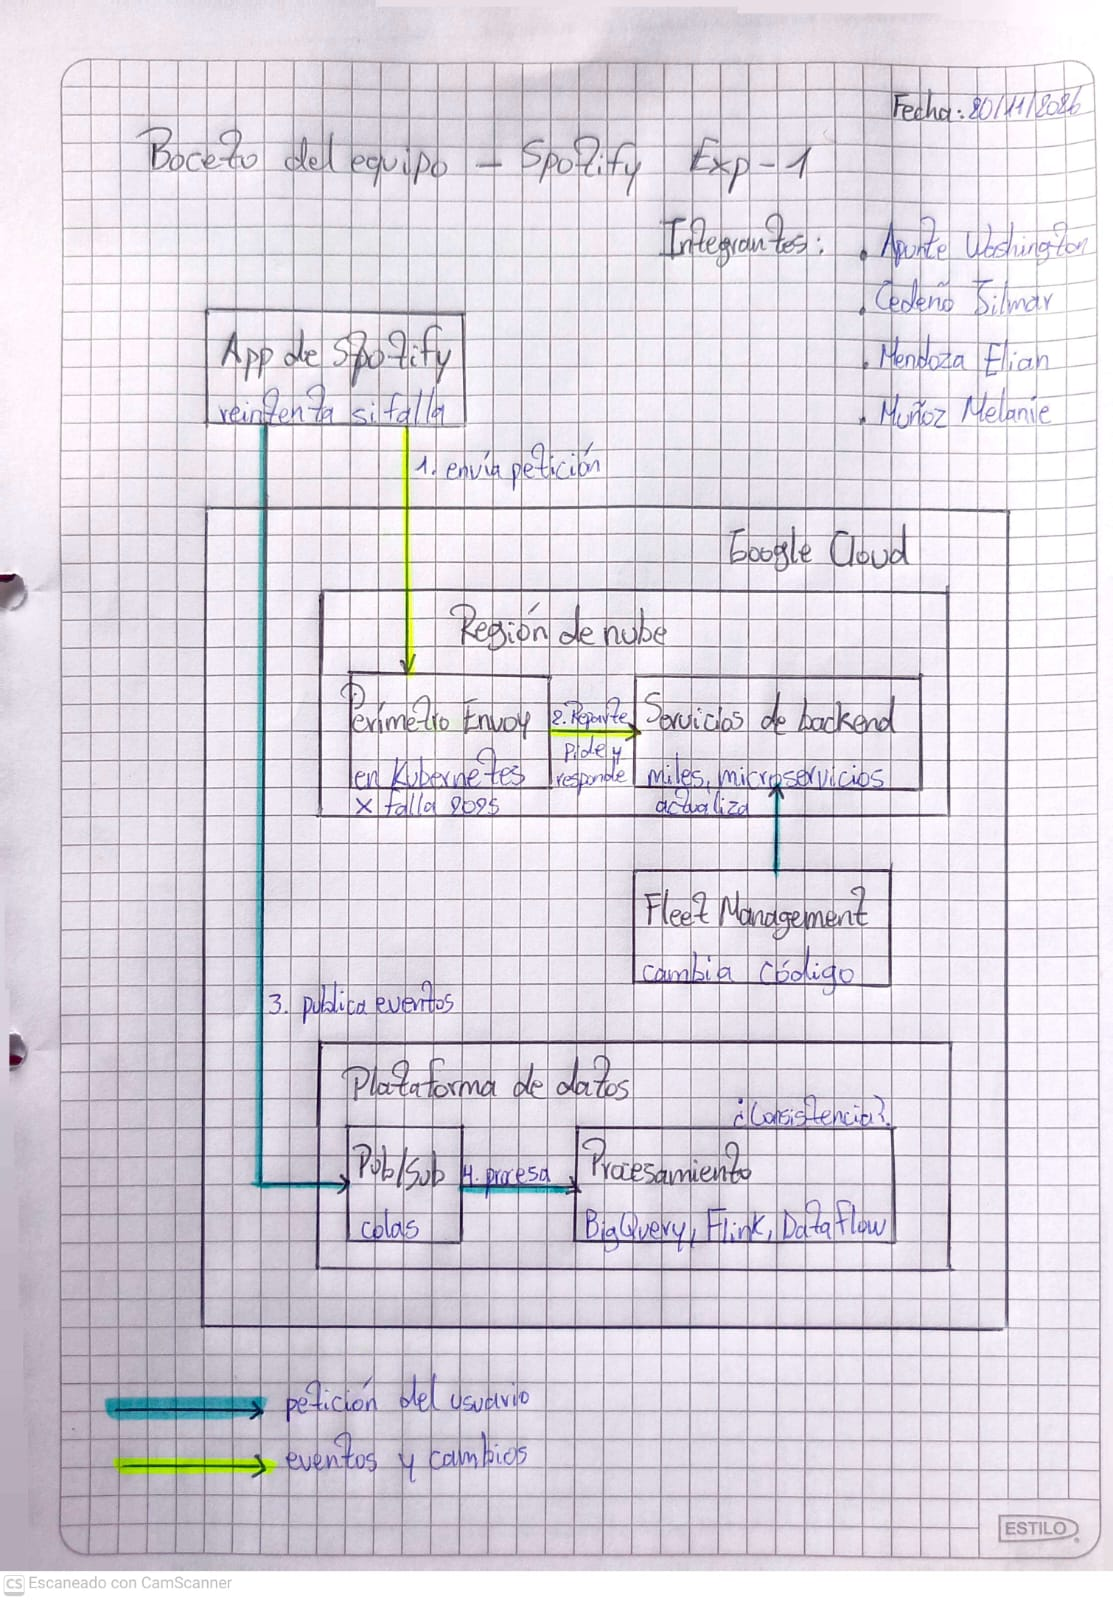
\includegraphics[width=\linewidth,height=0.76\textheight,keepaspectratio]{evidencias/boceto_equipo.jpg}
\end{center}
\end{document}
